%\documentclass[12pt,handout]{beamer}
%\documentclass{beamer}
\usepackage[ngerman]{babel}
\usepackage[utf8]{inputenc}
\usepackage{amsmath}
\usepackage{amssymb}
\usepackage{listings} 
\usepackage{stmaryrd}
\lstset{language=Python, tabsize=4, showstringspaces=false,basicstyle=\footnotesize,mathescape=true}  
\lstset{literate=%
  {Ö}{{\"O}}1
  {Ä}{{\"A}}1
  {Ü}{{\"U}}1
  {ß}{{\ss}}1
  {ü}{{\"u}}1
  {ä}{{\"a}}1
  {ö}{{\"o}}1
}
\usepackage{mathtools}
\usepackage{ulem}
\usepackage{tikz}

\usetheme{Boadilla}
\mode<presentation>{
\useoutertheme[subsection=false]{miniframes}
\useinnertheme{rectangles}
%\usecolortheme{crane}
}
\parskip 10pt



\begin{document}
\title{Informatik}   
\author{Graphen: Adjazenlisten, Tiefensuche, Zusammenhangskomponenten} 
\date{}
\frame{\titlepage} 

%---
\begin{frame}[fragile]
Implementation eines ungewichteten Graphen durch Adjazenzlisten, hier: Adjazenzmengen. 
Jedem Knoten wird in einem dictionary die Menge der Zielknoten der von ihm ausgehenden Kanten zugeordnet.
 
\begin{minipage}{5cm}
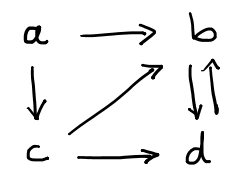
\includegraphics[scale=0.6]{bild30.png} 
\end{minipage} \pause
\begin{minipage}{5cm}
\begin{lstlisting} 
G = {'a':set('bc'),
     'b':set('d'), 
     'c':set('bd'),
     'd':set('b')}
\end{lstlisting}
\end{minipage} \pause

\begin{lstlisting} 
# gibt es Kante von a nach b  $\pause$
>>> 'b' in G['a']
True
# alle Nachbarn von a:  $\pause$
>>> for v in G['a']:
	print(v)
c
b
# alle Knoten von G durchlaufen: $\pause$
>>> for v in G:
       ....
\end{lstlisting}
\end{frame}

\begin{frame}[fragile]
Implementation eines gewichteten Graphen durch ein dictionary von dictionaries. Jedem Knoten wird ein dictionary zugeordnet, die jeder ausgehenden Kante ihre Kosten zuordnet.
 
\begin{minipage}{5cm}
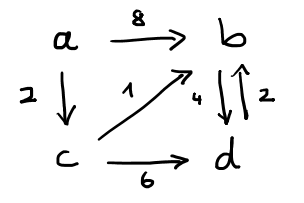
\includegraphics[scale=0.6]{bild31.png} 
\end{minipage} \pause
\begin{minipage}{5cm}
\begin{lstlisting} 
G = {'a': {'b':8, 'c':2},          
     'b': {'d':4},               
     'c': {'b':1, 'd':6},          
     'd': {'b':2}}
\end{lstlisting}
\end{minipage} \pause

\begin{lstlisting} 
 # gibt es Kante von a nach b  $\pause$
>>> 'b' in G['a']  
# die Kosten der Kante von a nach b:  $\pause$
>>> G['a']['b']     
# alle Nachbarn von a $\pause$
>>> for v in G['a']:   ....
# alle Knoten von G durchlaufen:  $\pause$
>>> for v in G:  ....

\end{lstlisting}
\end{frame}

%\begin{frame}[fragile]
%
%Analyse Implementation durch Adjazenzlisten: \pause
%
%Platzbedarf = $O(|E|)$.\\ \pause
%Bei Verwendung von Listen kein effizienter Zugriff auf Kante  $(x,y)$ möglich. \\ \pause
%Sinnvoll bei dünn besetzten Graphen, d.h. Graphen mit nur linear vielen Kanten. \\ \pause
%Sinnvoll bei Algorithmen, die, gegeben ein Knoten x, dessen Nachbarn verarbeiten müssen.
%
%\end{frame}
\begin{frame}[fragile]

\begin{minipage}[c]{5cm}
Erreichbarkeit

Gegeben ein Graph G und ein Startknoten s. Welche Knoten sind von s erreichbar?
\end{minipage}
\begin{minipage}[c]{6cm}
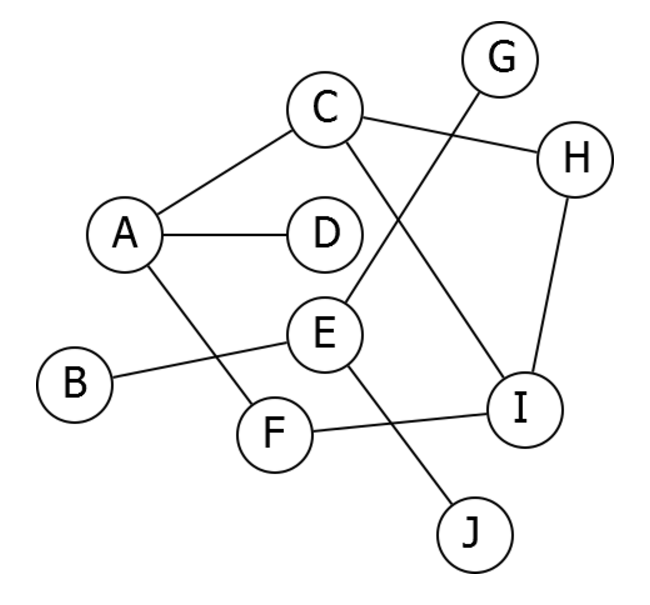
\includegraphics[width=5cm]{bild2.png}
\end{minipage}   \pause

\begin{lstlisting}
Setze alle Knoten auf nicht besucht
explore(s)
Gib alle Knoten aus, die besucht wurden

def explore(v): 
    merke v als besucht
    für alle Nachbarn w von v:
        wenn w nicht besucht:
            explore(w)

\end{lstlisting}

\end{frame}

\begin{frame}[fragile]

\begin{lstlisting}
visited =  {v : False for v in G}       
def explore(v):  
    visited[v] = True
    for w in G[v]:
        if not visited[w]:
            explore(w) 
 
explore(s)
result = [v for v in G if visited[v]]            
print(*result)
\end{lstlisting}   $\pause$
Die Funktion explore realisiert eine rekursive Tiefensuche (dfs, depth first search).

Laufzeit:  $\pause$ jeder Knoten wird höchstens einmal explored:  $O(\left|V\right|)$, jeder Knoten prüft seine Nachbarn, 
die Zahl der Nachbarn liegt in  $O(\left|E\right|)$, insgesamt also   $O(\left|V\right|+\left|E\right|)$.
\end{frame}

\begin{frame}[fragile]
Es gilt: Die Knoten eines ungerichteten Graphen G können in \textbf{Zusammenhangskomponenten} (Connected Components) aufgeteilt werden, so dass v von w genau dann erreichbar ist, wenn beide in derselben Zusammenhangskomponente liegen.

Bestimmung der Zusammenhangskomponenten:  

\begin{lstlisting} [basicstyle=\tiny]
Setze alle Knoten auf nicht besucht
Setze die Komponentennummer aller Knoten auf 0
cc = 1  # aktuelle Komponentennummer

Für alle Knoten u in G:
    falls u noch nicht besucht:
        explore(u)
        cc += 1
Gib Resultat aus 

def explore(v):
    merke v als besucht
    merke cc als Komponentennummer von v
    für alle Nachbarn w von v:
        wenn w nicht besucht:
            explore(w)

\end{lstlisting} 

\end{frame}

\begin{frame}[fragile]

\begin{lstlisting} [basicstyle=\scriptsize]
visited = {v : False for v in G}  
ccnum = {v : 0 for v in G}     # Komponentennummer von v
cc = 1                         # aktuelle Komponentennummer    

def explore(v):
    visited[v] = True
    ccnum[v] = cc
    for w in G[v]:
        if not visited[w]:
            explore(w)   

for v in G:
    if not visited[v] :
        explore(v)
        cc+=1 
      
for i in range(1,cc):
    result = [v for v in G if ccnum[v] $==$ i]   
    print(i,'-',*result)
\end{lstlisting} 

Laufzeit: $\pause O(\left|V\right|+\left|E\right|)$.
\end{frame}

\begin{frame}[fragile]
DFS endet damit, dass alle Knoten markiert sind. Das ist
als Ergebnis noch nicht sonderlich interessant. Interessant wird 
DFS daduch, dass man bei der Ausführung noch Daten sammelt, z.B. die previsit und postvisit Nummern.

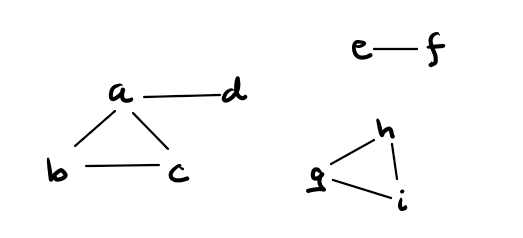
\includegraphics[width=9cm]{bild7.png}

\end{frame}

\begin{frame}[fragile]

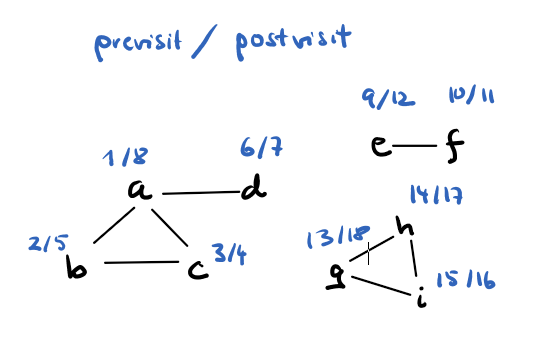
\includegraphics[width=8cm]{bild8.png}   $\pause$         

Für alle Knoten u und v gilt: die Intervalle [pre(u),post(u)] und [pre(v),post(v)] sind entweder
ineinander verschachtelt oder disjunkt.
\end{frame}

\begin{frame}[fragile]
Bestimmung der previsit und postvisit-Nummern der Tiefensuche
\begin{lstlisting} 
Setze alle Knoten auf nicht besucht
Setze previsit und postvisit Nummer aller Knoten auf 0
counter = 1  # Zähler für die visit-Nummer

Für alle Knoten u in G:
    falls u noch nicht besucht:
        explore(u)
Gib Resultat aus

def explore(v):
    merke v als besucht
    setze previsit-Nummer von v auf counter
    erhöhe counter um 1
    für alle Nachbarn w von v:
        wenn w nicht besucht:
            explore(w)
    setze postvisit-Nummer von v auf counter
    erhöhe counter um 1

\end{lstlisting} 
\end{frame}

\begin{frame}[fragile] 
\begin{lstlisting} [basicstyle=\scriptsize]
visited = {v : False for v in G}  
previsit = {v : 0 for v in G}         
postvisit = {v : 0 for v in G}     
counter = 1

def explore(v):
    global counter
    visited[v] = True
    previsit[v] = counter
    counter += 1
    for w in G[v]:
        if not visited[w]:
            explore(w)
    postvisit[v] = counter
    counter += 1

for v in G:
    if not visited[v] :
        explore(v)

for v in G:
    print("{:2} {:2} {:2}".format(v,previsit[v],postvisit[v]))
\end{lstlisting} 
\end{frame}

\begin{frame}[fragile] 
Topologische Sortierung eines gerichteten Graphen: wir wollen eine Nummerierung der Knoten finden, die mit den Kantenrichtungen
kompatibel ist.

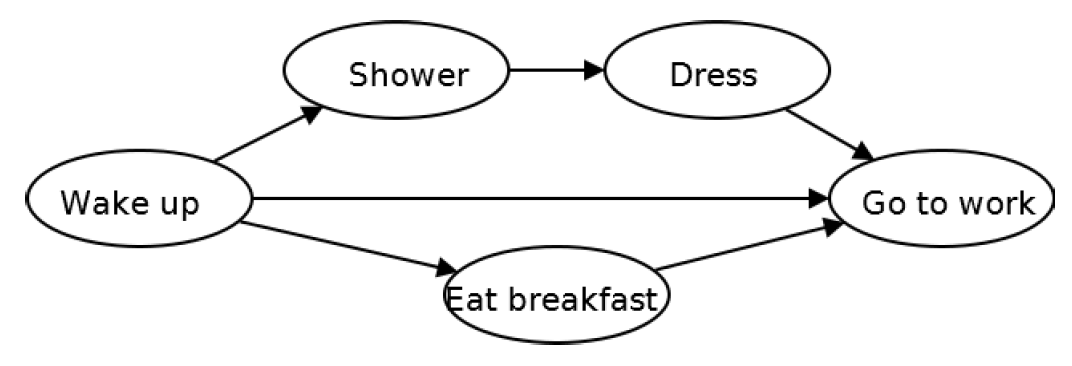
\includegraphics[width=7cm]{bild9.png} $\pause$         

Es gilt: ein Graph kann genau dann topologisch sortiert werden, wenn er keinen Kreis enthält.
Anders formuliert: Genau die gerichteten azyklischen Graphen (directed acyclic graph, DAG) können topologisch sortiert werden. 

\end{frame}

\begin{frame}[fragile] 
Eine Quelle (source) ist ein Knoten mit dem Eingangsgrad 0. Eine Senke (sink) ist ein Knoten mit dem Ausgangsgrad 0.

Bestimme die Senken des folgenden Graphen:

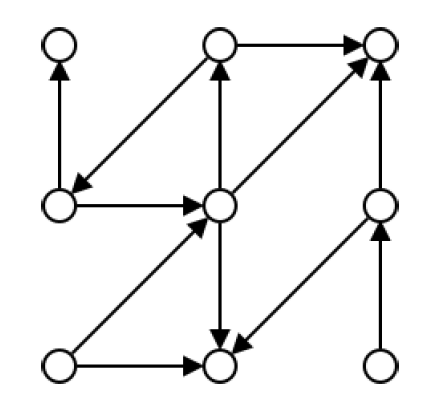
\includegraphics[width=6cm]{bild10.png}

\end{frame}

\begin{frame}[fragile] 

Idee für die topologische Sortierung (1. Versuch)
\begin{lstlisting} 
Solange der Graph nicht leer:
      Folge einem Pfad bis es nicht mehr weitergeht.
      Finde dort eine Senke
      Füge die Senke in die Sortierung wie in einen Stapel ein
      Entferne die Senke aus dem Graphen.


\end{lstlisting} 
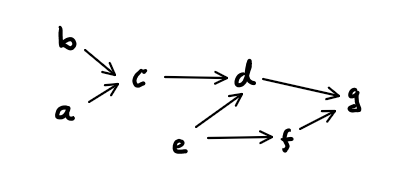
\includegraphics[width=6cm]{bild12.png}

Laufzeit: \pause $O(\left|V\right|^2)$    -   nicht gut

\end{frame}

\begin{frame}[fragile] 

Verbesserungsmöglichkeit: statt den Pfad immer wieder von vorne zu beginnen, wird nach der
Entfernung der Senke der Weg so weit wie nötig zurückgegangen 

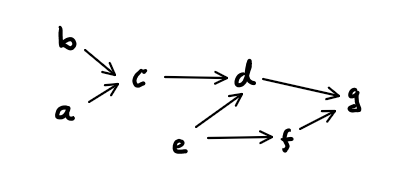
\includegraphics[width=6cm]{bild12.png}   \pause

Das ist Tiefensuche! 
Welche Nummerierung gibt uns eine topologische Sortierung? Zur Auswahl stehen:
previsit, postvisit, aufwärts, abwärts.  \pause
Die abwärts sortierte Reihe der postvisit-Nummern ergibt eine topologische Sortierung.
\end{frame}

\begin{frame}[fragile] 
\begin{lstlisting} 
visited = {v : False for v in G}  
postvisit = {v : 0 for v in G}     
counter = 1  

def explore(v):
    global counter
    visited[v] = True
    for w in G[v]:
        if not visited[w]:
            explore(w)
    postvisit[v] = counter
    counter += 1

for v in G:
    if not visited[v] :
        explore(v) 

result = sorted(G, key=lambda v: postvisit[v],reverse = True)
for i in range(len(result)):
    print(i+1,result[i])   
\end{lstlisting} 
\end{frame}

\begin{frame}[fragile] 
In einem gerichteten Graphen heißen zwei Knoten u und v \textbf{zusammenhängend}, wenn u von v und v von u erreichbar ist.  $\pause$         

Es gilt: Ein gerichteter Graph kann partitioniert werden in \textbf{starke Zusammenhangskomponenten} (strongly connected components (SCC)), wobei zwei Knoten genau dann zusammenhängen, wenn sie in der selben Komponente sind.
\end{frame}

\begin{frame}[fragile] 
Finde die starken Zusammenhangskomponenten in dem Graphen.

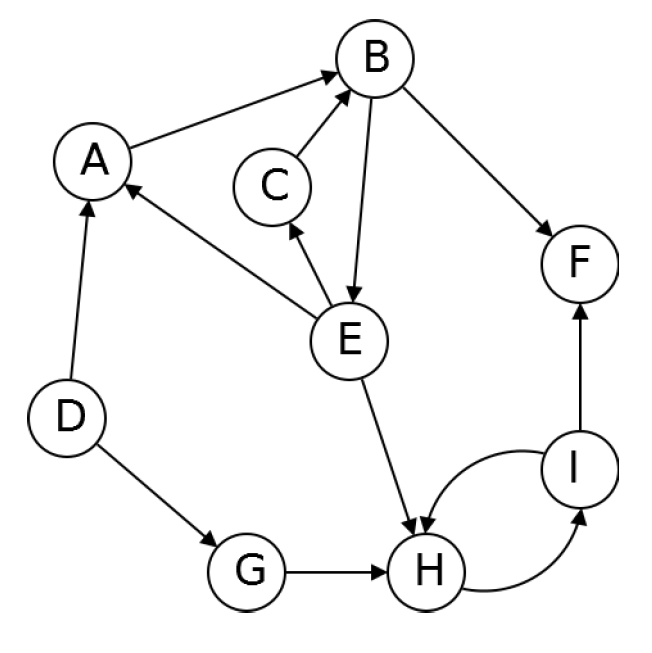
\includegraphics[width=6cm]{bild13.png}
\end{frame}

\begin{frame}[fragile] 

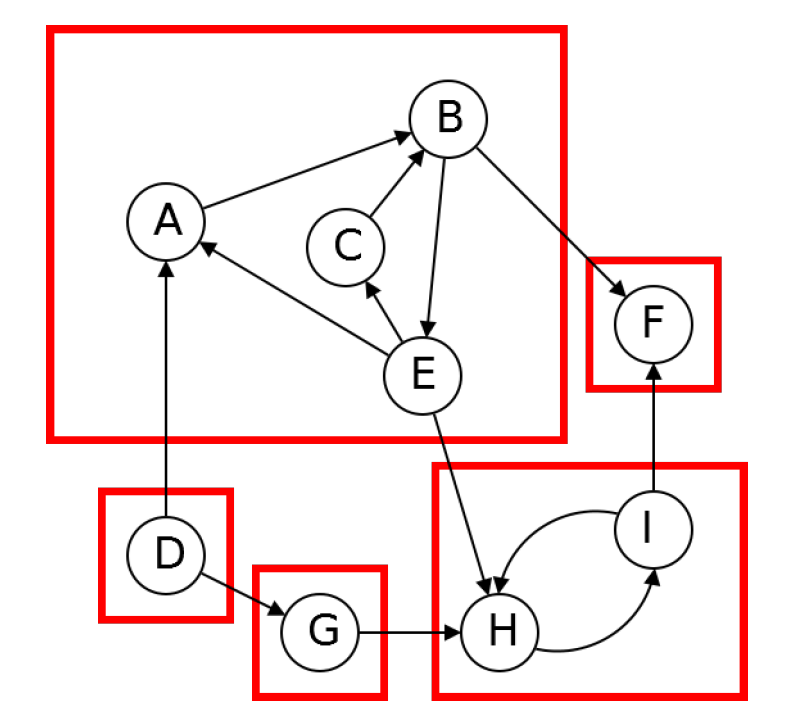
\includegraphics[width=7cm]{bild14.png}
\end{frame}

\begin{frame}[fragile] 
Der \textbf{Metagraph} zeigt, wie die starken Zusammenhangskomponenten untereinander verbunden sind.

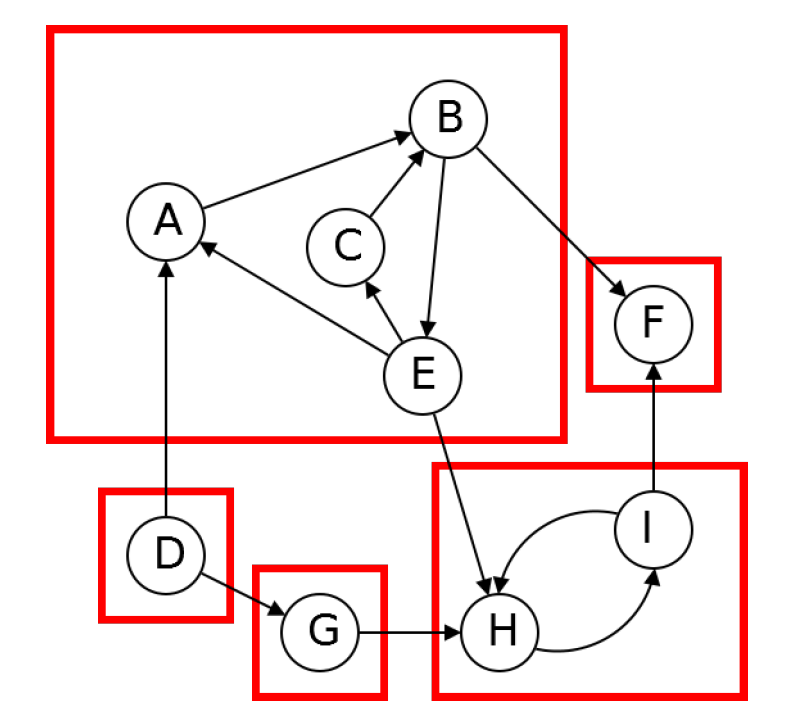
\includegraphics[width=5cm]{bild14.png}
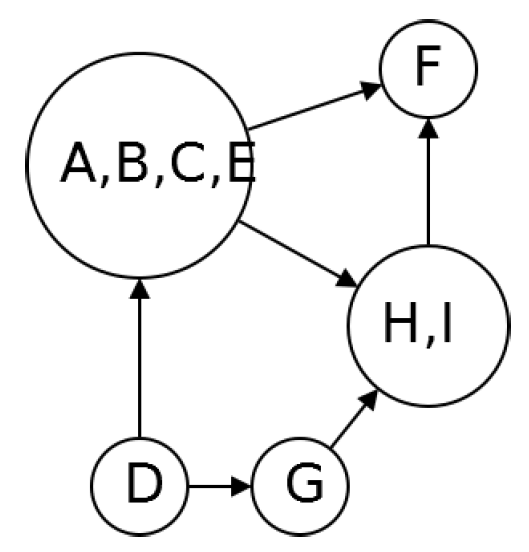
\includegraphics[width=4cm]{bild15.png}

Der Metagraph ist immer ein DAG.
\end{frame}

\begin{frame}[fragile] 
Wenn v in einer SCC-Senke liegt, dann findet explore(v) genau die Elemente des SCC.

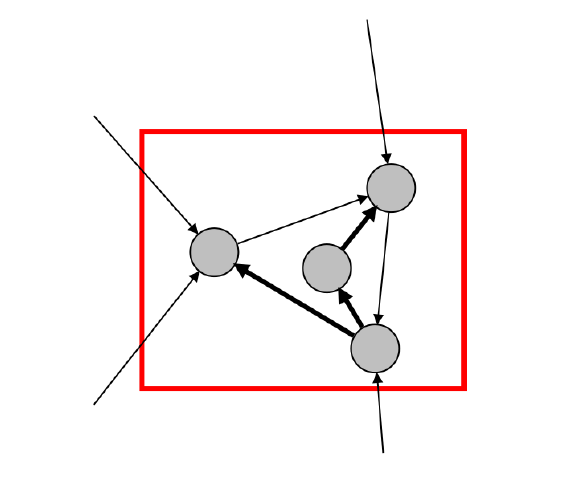
\includegraphics[width=6cm]{bild16.png}
\end{frame}

\begin{frame}[fragile] 
Es gilt: Wenn C und C' zwei starke Zusammenhangskomponenten sind und es eine Kante von einem Knoten aus C nach einem Knoten aus C' gibt, dann ist  die größte postvisit-Nummer in C größer als die größte postvisit-Nummer in C'. $\pause$    

Folgerung: der Knoten mit der größten postvisit-Nummer ist in einer SCC-Quelle. Wir suchen aber eine SCC-Senke. $\pause$    

Dazu betrachten wir den reversen Graphen. Den reversen Graphen $G^R$ eines gerichteten Graphen G erhält man, wenn
man die Kantenrichtungen umdreht. $\pause$    

$G$ und $G^R$ haben dieselben SCCs. \\
SCC-Quellen in $G^R$ sind SCC-Senken in $G$.

\end{frame}

\begin{frame}[fragile]
Bestimmung der postvisit-Nummern des reversen Graphen

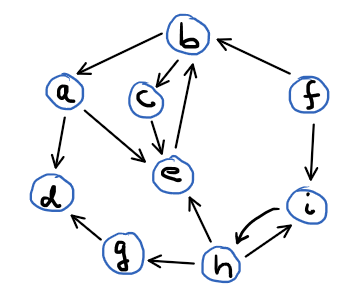
\includegraphics[width=5cm]{bild18.png} ~~  $\pause$    
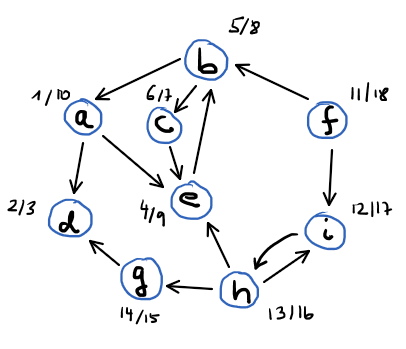
\includegraphics[width=5cm]{bild19.png} ~~  $\pause$    

Umgekehrte Reihenfolge der postvisit-Nummern: f i h g a e b c d

\end{frame}


\begin{frame}[fragile]
Bestimmung der SCCs mit Tiefensuche in der Reihenfolge  f i h g a e b c d.

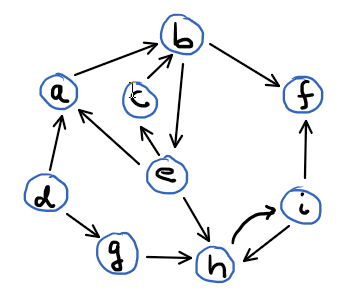
\includegraphics[width=5cm]{bild20.png} ~~  $\pause$    
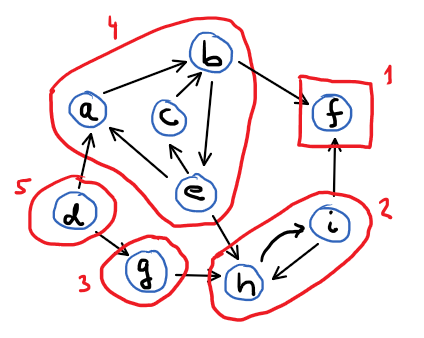
\includegraphics[width=5cm]{bild21.png} ~~  $\pause$   

Laufzeit: im wesentlichen Tiefensuche auf $G^R$ und dann auf $G$, also  $O(\left|V\right|+\left|E\right|)$.
\end{frame}

\begin{frame}[fragile]
Bestimmung der starken Zusammenhangskomponenten in einem gerichteten Graphen $G$
\begin{lstlisting} 
Führe Tiefensuche auf $G^R$ durch und merke postvisit-Nummern.
Für alle Knoten v in G in umgekehrter postvisit-Nummerierung:
	Falls v noch nicht besucht:
		explore(v) und markiere alle
			 besuchten Knoten u als neuen SCC.
             

\end{lstlisting} 
\end{frame}


\end{document}